\documentclass[10pt,letterpaper]{article}

\usepackage[T1]{fontenc}
\usepackage[utf8]{inputenc}
\usepackage{mathpazo}
\usepackage[scaled=0.92]{helvet}
\renewcommand{\ttdefault}{lmtt}
\usepackage{microtype}
\usepackage[margin=0.65in]{geometry}
\usepackage[table]{xcolor}
\usepackage{graphicx}
\usepackage{booktabs}
\usepackage{tabularx}
\usepackage{multirow}
\usepackage{array}
\usepackage{float}
\usepackage{placeins}
\usepackage{enumitem}
\usepackage{amsmath}
\usepackage{caption}
\usepackage{subcaption}
\usepackage{titlesec}
\usepackage{fancyhdr}
\usepackage{lastpage}
\usepackage[numbers,sort&compress]{natbib}
\usepackage[colorlinks=true,linkcolor=accent,citecolor=accent,urlcolor=accent]{hyperref}

\definecolor{accent}{RGB}{22,50,92}
\definecolor{muted}{RGB}{95,95,95}

\newcommand{\reportcourse}{CS 5326: Advanced Generative AI and Agents}
\newcommand{\reportassignment}{Programming Assignment 2}
\newcommand{\reporttitle}{Instruction Tuning and Direct Preference Optimization on a Small Language Model}
\newcommand{\reportinstructor}{Dr Agha Ali Raza}
\newcommand{\reportauthor}{Syed Muhammad Ashhar Shah}
\newcommand{\reportroll}{25030009}
\newcommand{\reportprogram}{MSCS}
\newcommand{\reportinstitution}{Lahore University of Management Sciences}

\hypersetup{pdftitle={\reportassignment: \reporttitle}, pdfauthor={\reportauthor}, pdfsubject={\reportcourse}}

\graphicspath{{assets/}}

\newcommand{\tablefont}{\footnotesize}

\titleformat{\section}{\sffamily\bfseries\small\MakeUppercase}{\thesection}{0.7em}{}
\titleformat{\subsection}{\sffamily\bfseries\small}{\thesubsection}{0.7em}{}
\titlespacing*{\section}{0pt}{1.6ex plus 0.3ex minus 0.2ex}{0.8ex plus 0.1ex}
\titlespacing*{\subsection}{0pt}{1.1ex plus 0.2ex minus 0.2ex}{0.5ex plus 0.1ex}
\titleformat{\paragraph}[runin]{\normalfont\normalsize\bfseries}{}{0pt}{}
\titlespacing*{\paragraph}{0pt}{1.2ex plus 0.2ex minus 0.1ex}{0.6em}
\hyphenation{UltraFeedback}

\captionsetup{font=footnotesize,labelfont={bf,sf},labelsep=period,skip=3pt}
\setlist{nosep,leftmargin=1.4em}
\setlength{\parindent}{1.2em}
\setlength{\parskip}{0pt}
\renewcommand{\baselinestretch}{0.97}
\setlength{\emergencystretch}{2em}
\setlength{\textfloatsep}{4pt plus 2pt minus 2pt}
\setlength{\floatsep}{6pt plus 2pt minus 2pt}
\setlength{\intextsep}{5pt plus 2pt minus 2pt}

\pagestyle{fancy}
\fancyhf{}
\fancyhead[L]{\sffamily\footnotesize\color{muted}\reportassignment: \reporttitle}
\fancyhead[R]{\sffamily\footnotesize\color{muted}\reportauthor}
\fancyfoot[L]{\sffamily\footnotesize\color{muted}\reportcourse}
\fancyfoot[R]{\sffamily\footnotesize\color{muted}Page \thepage\ of \pageref{LastPage}}
\renewcommand{\headrulewidth}{0.3pt}
\renewcommand{\footrulewidth}{0pt}
\fancypagestyle{firstpage}{\fancyhf{}\fancyfoot[L]{\sffamily\footnotesize\color{muted}\reportcourse}\fancyfoot[R]{\sffamily\footnotesize\color{muted}Page \thepage\ of \pageref{LastPage}}\renewcommand{\headrulewidth}{0pt}}

\makeatletter
\renewcommand\normalsize{\@setfontsize\normalsize{9.5}{11.4}}
\makeatother

\begin{document}

\thispagestyle{firstpage}
\begin{flushleft}
{\sffamily\bfseries\fontsize{17}{20.5}\selectfont \reportassignment:\\ Instruction Tuning and Direct Preference Optimization\\ on a Small Language Model\par}
\vspace{0.8em}
{\sffamily\bfseries\normalsize \reportauthor\par}
{\sffamily\small \reportprogram, Roll No.\ \reportroll, \reportinstitution\par}
{\sffamily\small \reportcourse; instructor: \reportinstructor\par}
\end{flushleft}
\vspace{0.3em}

\noindent{\sffamily\bfseries\small ABSTRACT}\par\vspace{2pt}
{\small\noindent This report follows a small post-training pipeline on Qwen2.5-0.5B: supervised fine-tuning (SFT) on 30,000 UltraChat examples, then two Direct Preference Optimization (DPO) runs written from scratch, one on 15,000 HH-RLHF pairs and one on 15,000 UltraFeedback pairs. A third experiment trains a LoRA persona adapter with TRL. I compare each DPO model with its SFT starting point on 300 fixed prompts, using a pairwise language-model judge. The HH-RLHF model beats SFT on its own safety prompts (win rate 0.596, $p=0.004$). The UltraFeedback model loses on AlpacaEval (0.392) because its answers are longer and repeat themselves more, and the loss turns into a tie (0.498) when I discourage repetition. The persona adapter either shows no persona or gains style at the cost of usefulness and safety. One judge, small evaluation sets, and a single training seed limit how far these conclusions reach.\par}
\vspace{0.4em}
\noindent{\sffamily\bfseries\small Additional Key Words and Phrases:} {\small preference optimization, DPO, supervised fine-tuning, LoRA, LLM-as-a-judge, small language models\par}
\vspace{0.2em}


\section{Repository, Models, and Data}
\label{sec:data}

The GitHub repository \url{https://github.com/AshharShah/small-model-alignment} holds all my code, configurations, metrics, generated responses, pairwise comparison files, and judged outputs. The limitations and reproducibility section lists the key paths.

\paragraph{Models.} The base checkpoint is Qwen/Qwen2.5-0.5B~\citep{qwen2025}. I fine-tuned it for SFT, then trained both DPO models from the best SFT checkpoint, which also serves as the frozen reference model in the DPO loss~\citep{rafailov2023dpo}. For the LoRA persona task, the assignment requires a different model, so I used the instruction-tuned HuggingFaceTB/\allowbreak SmolLM2-360M-Instruct~\citep{allal2025smollm2}.

\paragraph{Training and evaluation data.} Each training track has its own data (Table~\ref{tab:data}). SFT uses 30,000 training and 1,000 validation examples, each DPO run uses 15,000 training and 1,000 validation preference pairs, and the LoRA task uses 198 training and 22 validation pairs. Table~\ref{tab:evalsets} lists the four fixed evaluation sets: the course provides the HH set, and I built the other three. Within each comparison, I kept the evaluation prompts and their order fixed, so every model saw exactly the same inputs.

\begin{table}[H]
\centering
\caption{Training data per track. I shuffled every dataset with seed 42 before filtering.}
\label{tab:data}
\begingroup\small\renewcommand{\arraystretch}{1.12}
\begin{tabularx}{\textwidth}{>{\raggedright\arraybackslash}p{2.15cm}>{\raggedright\arraybackslash}p{4.3cm}p{2.2cm}>{\raggedright\arraybackslash}X}
\toprule
Track & Source (train / validation split) & Train / val & Filtering \\
\midrule
SFT & UltraChat-200k~\citep{ding2023ultrachat} (\texttt{train\_\allowbreak{}sft} / \texttt{test\_\allowbreak{}sft}) & 30,000 / 1,000 & first user--assistant turn only; prompt + response + EOS $\le$ 512 tokens (21,560 of 51,565 train rows dropped) \\
HH-RLHF DPO & HH-RLHF~\citep{bai2022hh} (\texttt{train} / \texttt{test}) & 15,000 / 1,000 & single-turn only (34,382 multi-turn rows dropped); prompt $\le$ 256 and prompt + response + EOS $\le$ 512 tokens (127 dropped) \\
UltraFeedback DPO & UltraFeedback, binarized~\citep{cui2023ultrafeedback,tunstall2023zephyr} (\texttt{train\_\allowbreak{}prefs} / \texttt{test\_\allowbreak{}prefs}) & 15,000 / 1,000$^\dagger$ & single-turn only; chosen score $>$ rejected (3,687 ties dropped); same length limits (12,124 dropped) \\
LoRA persona DPO & provided \texttt{ramsay\_\allowbreak{}style\_\allowbreak{}preferences.json} & 198 / 22 & none; seeded shuffle (seed 42), 22 rows held out \\
\bottomrule
\end{tabularx}
\endgroup

\par\vspace{3pt}\noindent\begin{minipage}{\textwidth}\footnotesize\raggedright $^\dagger$ 27 of the 1,000 validation pairs come from train rows that I did not use for training, because the test split has too few usable single-turn pairs.\end{minipage}
\end{table}

\begin{table}[H]
\centering
\caption{Fixed evaluation sets. ``Alignment tax'' means evaluating a DPO model on the other track's prompts.}
\label{tab:evalsets}
\begingroup\small\renewcommand{\arraystretch}{1.12}
\begin{tabularx}{\textwidth}{>{\raggedright\arraybackslash}p{2.3cm}r>{\raggedright\arraybackslash}X>{\raggedright\arraybackslash}p{4.1cm}}
\toprule
Evaluation set & Prompts & Composition & Used for \\
\midrule
AlpacaEval-300 & 300 & random subset (seed 42) of the 805 AlpacaEval prompts~\citep{dubois2024lc}: self-instruct 95, Koala 60, OASST 54, helpful\_base 51, Vicuna 40 & SFT vs.\ DPO-UF (main), DPO-HH (alignment tax) \\
HH-eval-300 & 300 & synthetic helpful/harmless set from the assignment; 10 categories $\times$ 30 prompts & SFT vs.\ DPO-HH (main), DPO-UF (alignment tax) \\
Persona-40 & 40 & hand-written; 4 categories $\times$ 10 prompts (cooking, coding, general help, safety-sensitive); no overlap with the training prompts & LoRA adapters vs.\ base model (test) \\
Held-out-22 & 22 & validation rows of the persona data that no training run used & LoRA adapter selection (dev) \\
\bottomrule
\end{tabularx}
\endgroup

\end{table}

\paragraph{Seeds, filtering and prompt format.} I used seed 42 everywhere to keep the experiments reproducible: for dataset shuffling and subset selection (including the AlpacaEval subset and the persona train/validation split), for every training run, and for the A/B order in the pairwise comparison files.

All Qwen runs share one prompt format, \texttt{\#\#\# Instruction:}\ $\langle$instruction$\rangle$\ \texttt{\#\#\# Response:}, with each marker on its own line and no chat template. This format covers SFT, both DPO runs, and every generation. SmolLM2 uses its own chat template for both training and generation.

I appended an EOS token to every training response and kept only the examples whose prompt, response, and EOS fit within 512 tokens. As a result, no example needed truncation and every response keeps its EOS label. I also kept only single-turn data: the first exchange of each UltraChat conversation, single-turn pairs from HH-RLHF and UltraFeedback, and DPO prompts of at most 256 tokens.


\section{Experimental Configuration}
\label{sec:config}

Table~\ref{tab:config} reports the values I used for the four submitted checkpoints, not the guide defaults. I generated every number in it from the saved configuration file of the matching run, so the table describes the submitted checkpoints exactly. I trained on Kaggle T4 GPUs, with the DPO policy on one GPU and its frozen reference on the other.

\begin{table}[H]
\centering
\caption{Configuration of the four submitted checkpoints. ``Kept'' marks the checkpoint I submitted.}
\label{tab:config}
\begingroup\tablefont\setlength{\tabcolsep}{3pt}\renewcommand{\arraystretch}{1.0}
\begin{tabularx}{\textwidth}{>{\raggedright\arraybackslash}p{1.8cm}>{\raggedright\arraybackslash}p{2.9cm}>{\raggedright\arraybackslash}p{2.9cm}>{\raggedright\arraybackslash}p{3.3cm}>{\raggedright\arraybackslash}p{2.4cm}>{\raggedright\arraybackslash}X}
\toprule
Run & Trainable parameters & Optimizer and schedule & Batch, precision, length, seed & DPO $\beta$ and reference & Generation \\
\midrule
SFT & full fine-tuning\newline (all weights) & AdamW, $\beta=(0.9,0.95)$\newline peak LR $2\times10^{-5}$\newline cosine to 0, warmup 28 steps (3\%)\newline weight decay 0.1, clip 1.0 & 2 $\times$ 16 accum.\ $=$ 32\newline fp32 weights, fp16 autocast\newline max length 512, seed 42\newline 1 epoch, 937 steps (kept: step~937) & n/a & greedy decoding\newline 512 new tokens\newline repetition penalty 1.0\newline length penalty 1.0\newline plain prompt template \\
HH-RLHF DPO & full fine-tuning\newline (all weights) & AdamW, $\beta=(0.9,0.95)$\newline peak LR $1\times10^{-6}$\newline constant, no warmup\newline weight decay 0, clip 1.0 & 1 pair $\times$ 32 accum.\ $=$ 32\newline fp32 weights, fp16 autocast (policy and reference)\newline max length 512, seed 42\newline 1 epoch, 468 steps (kept: step~400) & $\beta=0.1$\newline reference: frozen SFT best checkpoint (step~937) & greedy decoding\newline 512 new tokens\newline repetition penalty 1.0\newline length penalty 1.0\newline plain prompt template \\
UltraFeedback DPO & full fine-tuning\newline (all weights) & AdamW, $\beta=(0.9,0.95)$\newline peak LR $1\times10^{-6}$\newline constant, no warmup\newline weight decay 0, clip 1.0 & 1 pair $\times$ 32 accum.\ $=$ 32\newline fp32 weights, fp16 autocast (policy and reference)\newline max length 512, seed 42\newline 1 epoch, 468 steps (kept: step~468) & $\beta=0.1$\newline reference: frozen SFT best checkpoint (step~937) & greedy decoding\newline 512 new tokens\newline repetition penalty 1.0\newline length penalty 1.0\newline plain prompt template \\
LoRA-DPO (TRL) & LoRA $r=16$, $\alpha=32$, dropout 0.05\newline targets: q, k, v, o, gate, up, down & AdamW, default betas\newline peak LR $5\times10^{-5}$\newline cosine to 0, warmup 3 steps\newline weight decay 0, clip 1.0 & 4 $\times$ 4 accum.\ $=$ 16\newline fp32 weights, fp16 autocast\newline max length 512, seed 42\newline 3 epochs, 39 steps & $\beta=0.1$, plus NLL on the chosen answer\newline reference: base SmolLM2, adapter off & greedy decoding\newline 512 new tokens\newline repetition penalty 1.0\newline length penalty 1.0\newline SmolLM2 chat template \\
\bottomrule
\end{tabularx}
\endgroup

\end{table}

SFT and both DPO runs share the same optimizer, gradient clipping, maximum length, and seed. The two DPO runs differ only in their data: they start from the same SFT checkpoint, which also serves as their frozen reference. I kept the checkpoint with the best validation reward accuracy, which was step 400 of 468 for HH-RLHF and the final step for UltraFeedback. The best SFT checkpoint is also the final one (step 937).

The LoRA run differs in more than the data. It trains a LoRA adapter on SmolLM2 with TRL's \texttt{DPOTrainer}, using a larger learning rate, a smaller batch, and an extra negative log-likelihood (NLL) term on the chosen answer. The next section explains why I added that term.

\paragraph{Generation.} Every evaluation used greedy decoding (\texttt{do\_sample=False}), so temperature and top-p do not apply. I generated up to 512 new tokens with repetition penalty 1.0, length penalty 1.0, and no n-gram blocking, and I used identical settings for SFT and DPO within each comparison so that the judge compares models, not decoding policies. The Qwen runs use the plain prompt template from Section~\ref{sec:data}, and the SmolLM2 runs use the model's chat template.


\section{Parameter Choices and Deviations}
\label{sec:deviations}

For SFT and both DPO runs, I kept the guide recipe wherever nothing forced a change. Every headline hyperparameter in Table~\ref{tab:config} matches the guide tables, and so does the 256-token DPO prompt limit in Table~\ref{tab:data}. Table~\ref{tab:deviations} lists every other change, grouped by whether resource limits or performance evidence drove it.

\begin{table}[!t]
\centering
\caption{Changes from the guide, grouped by what drove them. ``My choice'' means the guide leaves the setting to me.}
\label{tab:deviations}
\begingroup\tablefont\setlength{\tabcolsep}{3pt}\renewcommand{\arraystretch}{1.0}
\begin{tabularx}{\textwidth}{>{\raggedright\arraybackslash}p{2.3cm}>{\raggedright\arraybackslash}p{2.5cm}>{\raggedright\arraybackslash}p{3.1cm}>{\raggedright\arraybackslash}X}
\toprule
Setting & Guide & Mine & Reason and effect \\
\midrule
\rowcolor{accent!8}\multicolumn{4}{@{}l}{\textbf{Resource-driven}} \\
SFT validation batch & not specified & 4, down from 8 & Validation ran out of memory on the T4. The loss is an exact token mean, so no value changes. \\
\rowcolor{accent!8}\multicolumn{4}{@{}l}{\textbf{Data and implementation choices}} \\
Long SFT examples & truncate to the maximum length & skip rows over 512 tokens until 30,000 fit & Truncation would cut the EOS label, so the model would never learn to stop. I did not test it. \\
DPO reference precision & fp16 allowed & fp32 weights under fp16 autocast & Memory allowed fp32, so policy and reference start identical. \\
\rowcolor{accent!8}\multicolumn{4}{@{}l}{\textbf{Performance-driven (LoRA persona task, where the guide leaves these settings to me)}} \\
Loss & plain DPO & DPO plus NLL on the chosen answer, weight 1 & Plain DPO left no persona (style 0/40/0). NLL gave small, mixed changes. \\
Learning rate & my choice & $5\times10^{-5}$ & The margin barely moved at $1\times10^{-5}$, and EOS collapsed from $7\times10^{-5}$ up (Table~\ref{tab:lorasweep}). \\
Epochs & my choice & 3 & Ten epochs raised style but cut EOS to 11/40, and the filter rejected it. \\
Rank & my choice & 16 (alpha 32) & Rank 8 reached half the margin at $5\times10^{-5}$ (0.52 against 1.02). I did not try it at a higher rate. \\
Targets and batch & my choice & all seven linear projections; 4 $\times$ 4 = 16 & Not ablated. A batch of 16 gives 13 updates per epoch, and 32 would give 7. \\
\bottomrule
\end{tabularx}
\endgroup

\end{table}

\paragraph{Resource-driven changes.} The memory problem I hit was in SFT validation, not in training. Validation ran out of memory on the T4, where training itself peaked at 12.8 GB, so I halved the validation batch from 8 to 4 and set the expandable-segments allocator. Validation loss is an exact token mean, so the batch size changes no value. Memory never forced a training change: SFT and DPO ran at the guide batch sizes without gradient checkpointing.

\paragraph{Data and implementation choices.} Three choices differ from the guide without anything forcing them. The guide truncates long SFT examples to 512 tokens, and I skipped them instead (21,560 of the 51,565 rows I read) until 30,000 fit, because truncation would cut the EOS label and the model would never learn to stop. The guide lets the DPO reference load in fp16, and I used fp32: it needed only 3.4 to 4.2 GB on its own T4, and policy and reference then start identical, with the largest absolute implicit reward at step 0 at $2.4\times10^{-5}$ for HH-RLHF and $4.3\times10^{-5}$ for UltraFeedback.

\paragraph{LoRA settings.} The guide leaves the LoRA settings to me, so these are the performance-driven choices, and I made them by training 12 adapters in two sweeps (Table~\ref{tab:lorasweep}). Plain DPO at $5\times10^{-5}$ gave no persona on the 40 required prompts (0 wins, 40 ties, 0 losses), so I added the NLL term on the chosen answer. It changed little: held-out EOS went from 19 to 20 of 22, and required-prompt EOS from 40 to 35 of 40. At $1\times10^{-5}$ the validation margin barely moved (0.12), and from $7\times10^{-5}$ up the answers degraded: required-prompt EOS fell from 40 of 40 at $5\times10^{-5}$ to 31, 30, and 2 of 40 at $7\times10^{-5}$, $1\times10^{-4}$, and $2\times10^{-4}$. More epochs did the same. Ten epochs at $5\times10^{-5}$ gave the strongest plain-DPO style (9 wins, 31 ties, 0 losses), but EOS fell to 11 of 40, and my filter rejected it. I chose rank 16 over rank 8 because rank 8 reached only half the margin at $5\times10^{-5}$ (0.52 against 1.02), though I did not try it at a higher rate. I did not ablate the target modules or the batch size (Table~\ref{tab:deviations}).

\paragraph{Which adapters I scored.} The dashes in Table~\ref{tab:lorasweep} show which checks each adapter went through. In the first sweep, I trained seven plain-DPO adapters for three epochs and generated answers only for the 40 required prompts, which gives their EOS and loop counts. I judged style for two of them (the $5\times10^{-5}$ and $1\times10^{-4}$ runs) and generated held-out answers only for the $5\times10^{-5}$ run. The second sweep added five adapters with more epochs or the NLL term, and I scored each on both prompt sets and judged its style. I did not take the other six first-sweep adapters further. Four of them, at learning rates of $7\times10^{-5}$ and above, already break the filter's thresholds on the 40 required prompts alone, which the table marks as ``fail on the 40 alone''. The other two, at $1\times10^{-5}$ and with rank 8, trained the smallest margins (0.12 and 0.52).

\paragraph{Adapter selection.} Before I scored any adapter on the held-out prompts, I fixed the selection rule. An adapter fails if, on either prompt set, its EOS rate falls by more than 10 points or its repeated-phrase rate rises by more than 10 points relative to the base model. Among the adapters that pass, I take the highest held-out style score. Only one of the six adapters I scored on both prompt sets passed, so I selected rank 16, a learning rate of $5\times10^{-5}$, three epochs, and the NLL term. That choice has a cost: the adapters that move the persona style most all fail the filter, and the one that passes barely moves it. Section~\ref{sec:results} reports both.

\begin{table}[!t]
\centering
\caption{All 12 adapters I trained for the persona task, in two sweeps. The columns marked 40 and the style column use the 40 required prompts, and the columns marked 22 use the 22 held-out prompts. EOS counts answers that end on their own, loops counts answers with a repeated phrase, and Style W/T/L is the judge's persona-style win, tie, and loss count against the base model. A dash means I did not run that check. The filter needs both prompt sets, so ``fail on the 40 alone'' marks adapters that already break its 10-point thresholds on the required prompts. Shading marks the selected adapter.}
\label{tab:lorasweep}
\begingroup\tablefont\setlength{\tabcolsep}{3pt}\renewcommand{\arraystretch}{1.0}
\begin{tabularx}{\textwidth}{>{\centering\arraybackslash}p{0.8cm}>{\centering\arraybackslash}p{1.4cm}>{\centering\arraybackslash}p{1.0cm}>{\centering\arraybackslash}p{1.9cm}>{\centering\arraybackslash}p{1.2cm}>{\centering\arraybackslash}p{1.2cm}>{\centering\arraybackslash}p{1.2cm}>{\centering\arraybackslash}p{1.2cm}>{\centering\arraybackslash}p{1.2cm}>{\centering\arraybackslash}p{1.7cm}>{\raggedright\arraybackslash}X}
\toprule
Rank & Learning rate & Epochs & Loss & Val. margin & EOS of 40 & Loops of 40 & EOS of 22 & Loops of 22 & Style W/T/L & Filter \\
\midrule
\multicolumn{5}{@{}l}{Base model, no adapter} & 37/40 & 11 & 22/22 & 2 & - & - \\
16 & $1\times10^{-5}$ & 3 & DPO & 0.12 & 38/40 & 12 & - & - & - & - \\
8 & $5\times10^{-5}$ & 3 & DPO & 0.52 & 39/40 & 11 & - & - & - & - \\
16 & $5\times10^{-5}$ & 3 & DPO & 1.02 & 40/40 & 11 & 19/22 & 5 & 0/40/0 & fail \\
16 & $7\times10^{-5}$ & 3 & DPO & 1.55 & 31/40 & 15 & - & - & - & fail on the 40 alone \\
16 & $1\times10^{-4}$ & 3 & DPO, $\beta=0.3$ & 5.17 & 33/40 & 20 & - & - & - & fail on the 40 alone \\
16 & $1\times10^{-4}$ & 3 & DPO & 2.30 & 30/40 & 24 & - & - & 2/38/0 & fail on the 40 alone \\
16 & $2\times10^{-4}$ & 3 & DPO & 5.47 & 2/40 & 38 & - & - & - & fail on the 40 alone \\
16 & $5\times10^{-5}$ & 10 & DPO & 4.79 & 11/40 & 33 & 3/22 & 20 & 9/31/0 & fail \\
\rowcolor{accent!10}16 & $5\times10^{-5}$ & 3 & DPO + NLL & 0.96 & 35/40 & 13 & 20/22 & 3 & 0/40/0 & pass (selected) \\
16 & $1\times10^{-4}$ & 3 & DPO + NLL & 2.07 & 28/40 & 18 & 10/22 & 12 & 1/39/0 & fail \\
16 & $5\times10^{-5}$ & 6 & DPO + NLL & 2.21 & 32/40 & 17 & 10/22 & 12 & 1/39/0 & fail \\
16 & $1\times10^{-4}$ & 6 & DPO + NLL & 3.59 & 33/40 & 12 & 15/22 & 9 & 24/16/0 & fail \\
\bottomrule
\end{tabularx}
\endgroup

\end{table}


\section{Training Behavior}
\label{sec:training}

Figure~\ref{fig:training} plots the SFT run and both DPO runs. The training curves are noisy, because each point comes from a single batch of 32, so I judge convergence from the validation measurements: 1,000 held-out examples for SFT and 1,000 held-out preference pairs for each DPO run.

\begin{figure}[!t]
\centering
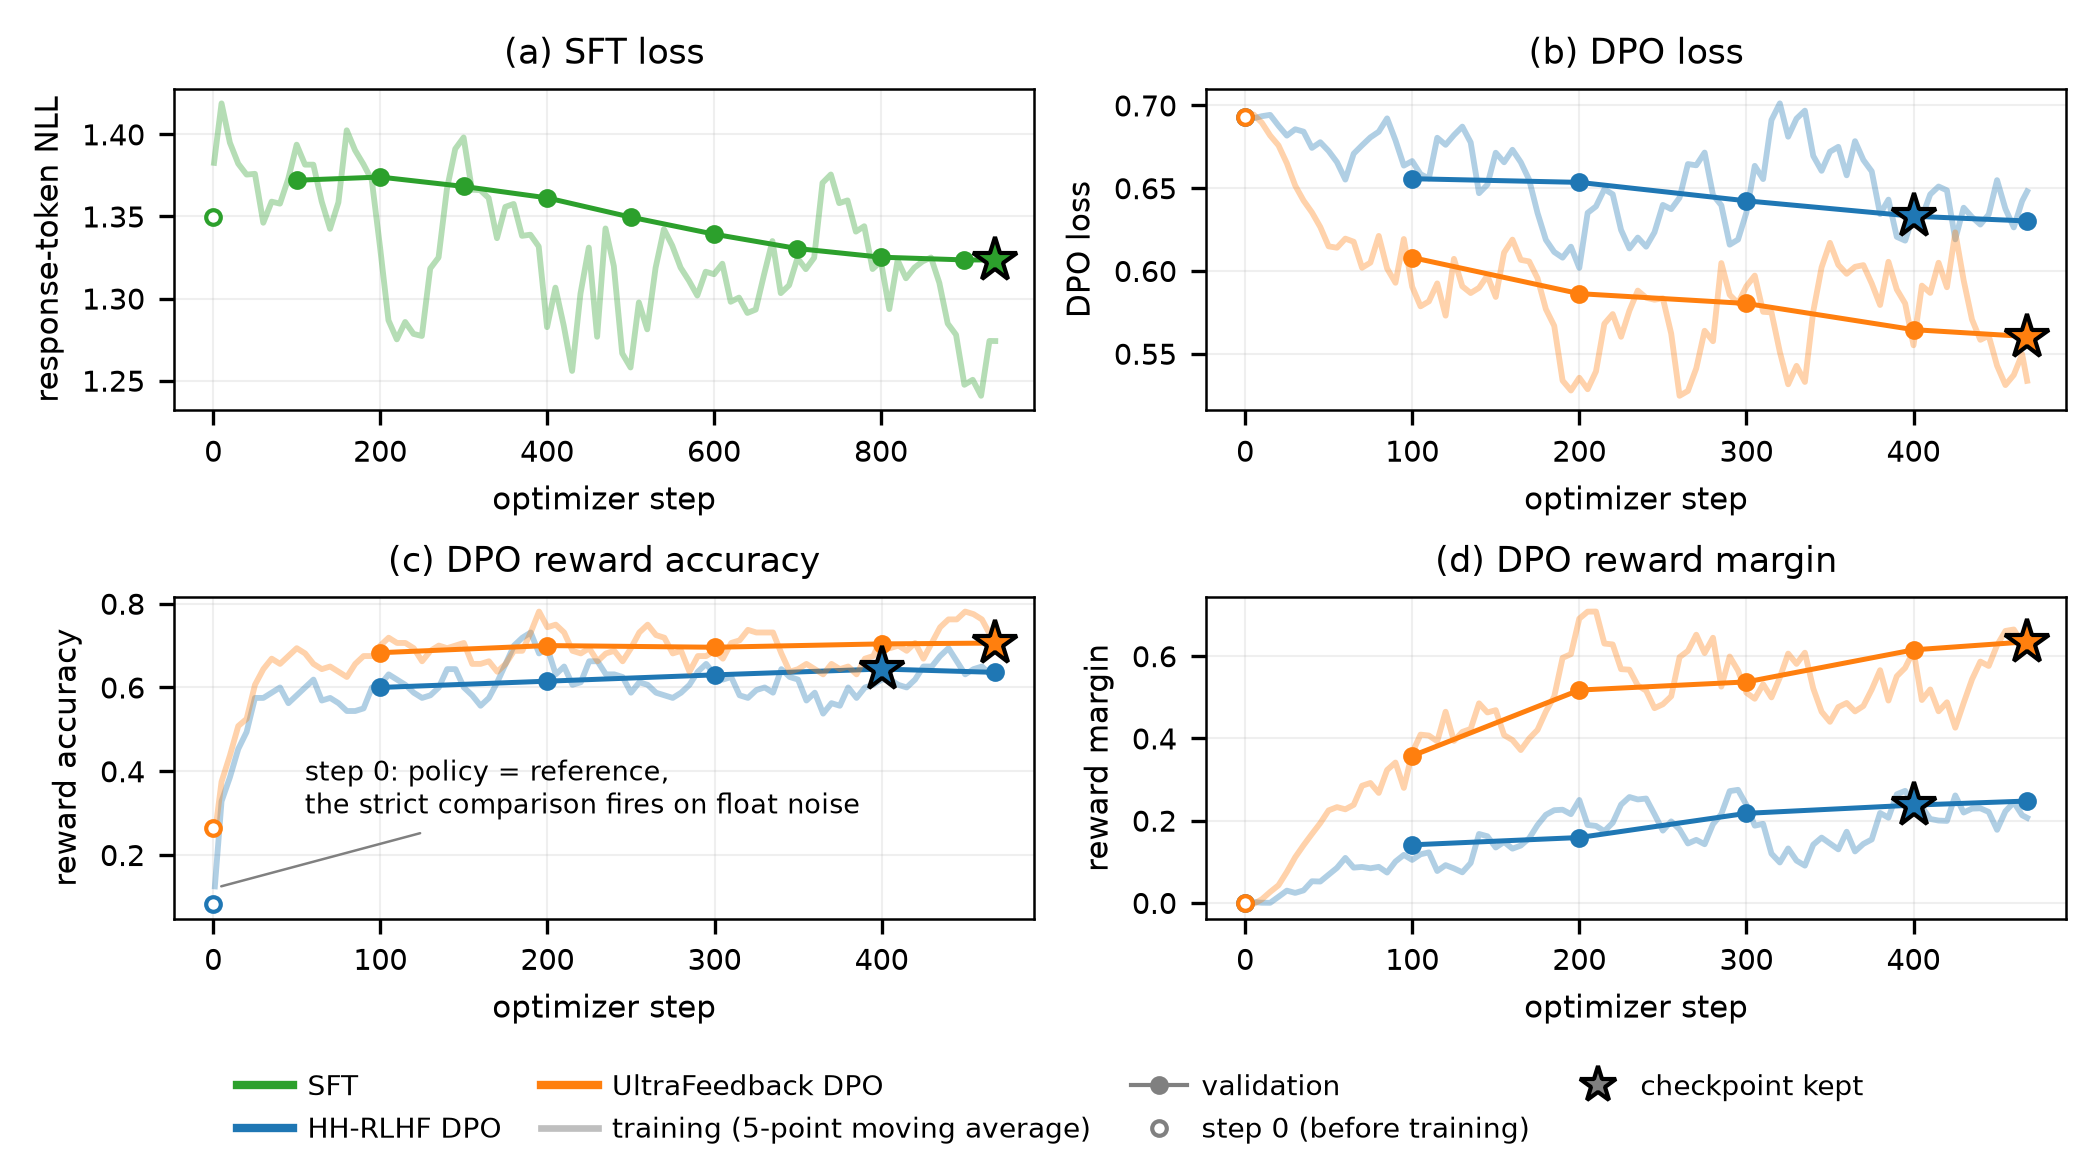
\includegraphics[width=0.84\textwidth]{assets/fig_training.png}
\caption{Training curves for SFT (a) and both DPO runs (b--d). Thin faded lines show training metrics, which I logged every 10 optimizer steps (SFT) or every 5 (DPO) and smoothed with a 5-point moving average. Dots show validation metrics at every 100 steps and at the last step. Hollow dots mark step 0, before any update, and stars mark the checkpoint I kept. In (c), the step-0 accuracy is an artifact: the policy equals the reference, so the two rewards differ only by floating-point noise.}
\label{fig:training}
\end{figure}

\paragraph{SFT.} Validation loss rose slightly from 1.350 at step 0 to 1.374 at step 200, then fell at every later evaluation to 1.323 at step 937 (perplexity 3.86 to 3.76). It never turned upward, so one epoch showed no sign of overfitting, and the best checkpoint is the final one. Training loss falls from a mean of 1.37 over the first ten logged steps to 1.28 over the last ten, and with one epoch every batch is new when I score it, so it behaves like a held-out loss.

\paragraph{DPO.} Both runs start at a loss of $\ln 2 \approx 0.693$, the value when the policy equals the reference. HH-RLHF improves slowly: validation loss falls from 0.656 at step 100 to 0.630 at the end, reward accuracy creeps from 0.60 to 0.64, and the reward margin grows from 0.14 to 0.25. UltraFeedback separates its pairs much more easily: validation loss falls from 0.608 to 0.560, accuracy rises from 0.68 to 0.71, and the margin grows from 0.36 to 0.63. Training and validation agree. Over the last 100 steps, training reward accuracy was 0.63 for HH-RLHF and 0.72 for UltraFeedback, against validation accuracies of 0.636 and 0.706, so I see no overfitting in either run. The UltraFeedback margin was still rising when the epoch ended, so that run had not converged.

\paragraph{Checkpoint selection.} I kept the checkpoint with the highest validation reward accuracy: step 400 (0.644) for HH-RLHF and the final step (0.706) for UltraFeedback. For HH-RLHF, step 400 beats the final step 468 (0.636) by only 0.8 points, which is less than the roughly 1.5-point binomial standard error of either number, and validation loss is marginally lower at step 468 (0.630 against 0.633). I therefore treat the two checkpoints as equivalent, and I see step 400 as a tie-break, not as evidence of overfitting.

\paragraph{Stability.} No run diverged. The only instability was fp16 overflow early in both DPO runs: the loss scaler halved three times, from 65,536 to 8,192, within the first 175 steps of each run, so I infer that it skipped three of the 468 updates in each run. SFT never overflowed.

\paragraph{Implicit rewards.} On the validation pairs, the implicit rewards of both the chosen and the rejected answers fell below zero in both runs (final values: $-0.30$ and $-0.55$ for HH-RLHF, $-0.12$ and $-0.75$ for UltraFeedback). The margin grows because the policy lowers the probability of rejected answers more than that of chosen ones, not because it raises the probability of chosen ones. Figure~\ref{fig:behavior}c and d plot both scores.

\paragraph{LoRA.} The LoRA run has only 39 updates on 198 pairs, too few for a curve. On its 22 validation pairs, the selected adapter reaches a reward accuracy of 1.0 and a margin of 0.96, which shows it separates the persona answer from the plain one, not that its generations change style.

None of these curves measures response quality. They show how well each model separates pairs from its own preference data, so I judge the checkpoints on generated responses, as the next section reports.


\section{DPO-versus-SFT Results}
\label{sec:results}

For each DPO track, I compared the submitted checkpoint with the SFT checkpoint it started from, on the same 300 prompts, with the same generation settings and the same judge (Table~\ref{tab:dpo}). I report each comparison separately and never average across them. The two tracks use different prompts, rubrics, and preference data, so a single headline score would mix unlike targets.

\begin{table}[!t]
\centering
\caption{Pairwise judge results for each DPO model against SFT on identical prompts: wins (W), ties (T), losses (L), unknown verdicts (Unk.), and judge calls beyond one per batch of five (extra calls). Win rate excluding ties is W/(W+L) with a 95\% Wilson interval, win rate with ties counts each tie as half a win, and the sign test is exact and two-sided on W against L. The plain rubric drops the length guidance, and the repetition penalty applies to both models.}
\label{tab:dpo}
\begingroup\tablefont\setlength{\tabcolsep}{3pt}\renewcommand{\arraystretch}{1.0}
\begin{tabularx}{\textwidth}{>{\raggedright\arraybackslash}X>{\centering\arraybackslash}p{0.7cm}>{\centering\arraybackslash}p{0.7cm}>{\centering\arraybackslash}p{0.7cm}>{\centering\arraybackslash}p{0.7cm}>{\centering\arraybackslash}p{0.8cm}>{\centering\arraybackslash}p{1.0cm}>{\centering\arraybackslash}p{3.0cm}>{\centering\arraybackslash}p{1.4cm}>{\centering\arraybackslash}p{1.2cm}}
\toprule
Comparison & n & W & T & L & Unk. & Extra calls & Win rate, ties excluded [95\% CI] & Win rate, ties $\tfrac{1}{2}$ & Sign test $p$ \\
\midrule
\rowcolor{accent!8}\multicolumn{10}{@{}l}{\textbf{Own-track comparison: submitted DPO checkpoint against its SFT baseline}} \\
HH-RLHF DPO vs SFT, HH-eval & 300 & 137 & 70 & 93 & 0 & 8 & 0.596 [0.531, 0.657] & 0.573 & 0.004 \\
UltraFeedback DPO vs SFT, AlpacaEval & 300 & 94 & 60 & 146 & 0 & 1 & 0.392 [0.332, 0.455] & 0.413 & 0.001 \\
\rowcolor{accent!8}\multicolumn{10}{@{}l}{\textbf{Alignment tax: the other track's prompts}} \\
HH-RLHF DPO vs SFT, AlpacaEval & 300 & 102 & 93 & 105 & 0 & 2 & 0.493 [0.425, 0.560] & 0.495 & 0.889 \\
UltraFeedback DPO vs SFT, HH-eval & 300 & 96 & 68 & 134 & 2 & 20 & 0.417 [0.355, 0.482] & 0.436 & 0.015 \\
\rowcolor{accent!8}\multicolumn{10}{@{}l}{\textbf{Sensitivity of the own-track comparisons (HH-RLHF DPO on HH-eval, UltraFeedback DPO on AlpacaEval): one setting changed}} \\
HH-eval, positions swapped & 300 & 147 & 60 & 93 & 0 & 4 & 0.613 [0.550, 0.672] & 0.590 & <0.001 \\
HH-eval, plain rubric & 300 & 134 & 68 & 97 & 1 & 12 & 0.580 [0.516, 0.642] & 0.562 & 0.018 \\
HH-eval, repetition penalty 1.1 & 300 & 133 & 71 & 96 & 0 & 3 & 0.581 [0.516, 0.643] & 0.562 & 0.017 \\
AlpacaEval, positions swapped & 300 & 94 & 75 & 131 & 0 & 3 & 0.418 [0.355, 0.483] & 0.438 & 0.016 \\
AlpacaEval, plain rubric & 300 & 97 & 65 & 138 & 0 & 4 & 0.413 [0.352, 0.477] & 0.432 & 0.009 \\
AlpacaEval, repetition penalty 1.1 & 300 & 121 & 57 & 122 & 0 & 4 & 0.498 [0.436, 0.560] & 0.498 & 1.000 \\
\bottomrule
\end{tabularx}
\endgroup

\end{table}

\paragraph{Results.} On its own track, HH-RLHF DPO beat SFT on the HH-eval prompts, with 137 wins, 70 ties, and 93 losses. That is a win rate of 0.596 excluding ties (95\% interval 0.531 to 0.657) and 0.573 counting ties as half a win. UltraFeedback DPO lost to SFT on AlpacaEval, with 94 wins, 60 ties, and 146 losses, or 0.392 (0.332 to 0.455) and 0.413. Both gaps pass the sign test ($p=0.004$ and $0.001$). On the other track's prompts, HH-RLHF DPO matched SFT on AlpacaEval (102 wins, 93 ties, 105 losses; 0.493, $p=0.889$) and gave exactly SFT's answer on 30 of the 300 prompts, while UltraFeedback DPO lost on HH-eval (96, 68, 134; 0.417, $p=0.015$).

\paragraph{Judging procedure.} The judge is google/gemini-3.6-flash. It saw five prompts per request, with the two responses to each prompt in a seeded random A/B order (each model came first in exactly 150 of the 300 pairs) and no model names, and it answered A, B, or tie. The rubric matches the track: helpfulness and correctness for AlpacaEval, with a safety addendum for HH-eval. Both rubrics tell the judge not to prefer an answer for its length alone.

\paragraph{Failures and invalid verdicts.} I retried a failed request up to three times with a 5\,s pause, and then re-asked the pairs of a failed batch one at a time. A verdict that stayed invalid after that counts as unknown, and I excluded it from both win rates and logged it in a failure file. Only UltraFeedback DPO on the HH-eval prompts ended with unknown verdicts (2 of 300, after 3 failed batches and 20 extra calls), and a separate retry run did not resolve them. The plain-rubric check on HH-eval has one more. Pairs with identical outputs count as ties without a judge call, which covered 5 of the 300 UltraFeedback pairs and 2 of the 300 HH-RLHF pairs.

\paragraph{Sensitivity.} Swapping the A/B positions and removing the rubric's length guidance leave both conclusions in place: HH-RLHF scores 0.613 and 0.580, and UltraFeedback 0.418 and 0.413. A repetition penalty of 1.1, applied to both models, leaves HH-RLHF almost unchanged (133 wins, 71 ties, 96 losses; 0.581) but lifts UltraFeedback from 0.392 to 0.498 (121 wins, 57 ties, 122 losses), a tie ($p=1.0$). The UltraFeedback deficit therefore depends on the decoding setting, and the next section returns to why.

\paragraph{LoRA persona result.} The persona task has a different target, so I report it on its own (Table~\ref{tab:lorares}) and do not combine it with the DPO numbers. I judged each adapter against the base SmolLM2 model on persona style, usefulness, and safety. As a positive control, the judge compared the dataset's persona answers with its neutral answers on the 22 held-out prompts and picked the persona answer all 22 times, so the style rubric can see the persona. The selected adapter does not change the style the judge sees (0 wins and 40 ties on the required prompts, 2 wins and 20 ties on the held-out prompts), and its usefulness (16 wins, 3 ties, 21 losses) and safety (4, 32, 4) are not significantly different from the base model ($p=0.511$ and $1.0$). The strongest persona adapter, which used twice the learning rate and twice the epochs, wins on style (24 wins, 16 ties, 0 losses on the required prompts; 19, 3, 0 on the held-out prompts) but loses on usefulness (11, 2, 27; $p=0.014$) and safety (4, 18, 18; $p=0.004$). No LoRA verdict was unknown.

\begin{table}[!t]
\centering
\caption{LoRA persona results, each adapter against the base SmolLM2 model, one rubric per target. Table~\ref{tab:dpo} defines the columns.}
\label{tab:lorares}
\begingroup\tablefont\setlength{\tabcolsep}{3pt}\renewcommand{\arraystretch}{1.0}
\begin{tabularx}{\textwidth}{>{\raggedright\arraybackslash}X>{\centering\arraybackslash}p{0.7cm}>{\centering\arraybackslash}p{0.7cm}>{\centering\arraybackslash}p{0.7cm}>{\centering\arraybackslash}p{0.7cm}>{\centering\arraybackslash}p{3.0cm}>{\centering\arraybackslash}p{1.4cm}>{\centering\arraybackslash}p{1.2cm}}
\toprule
Judged target & n & W & T & L & Win rate, ties excluded [95\% CI] & Win rate, ties $\tfrac{1}{2}$ & Sign test $p$ \\
\midrule
\rowcolor{accent!8}\multicolumn{8}{@{}l}{\textbf{Positive control}} \\
Dataset persona answers vs neutral answers: style, 22 held-out prompts & 22 & 22 & 0 & 0 & 1.000 [0.851, 1.000] & 1.000 & <0.001 \\
\rowcolor{accent!8}\multicolumn{8}{@{}l}{\textbf{Selected adapter: rank 16, learning rate $5\times10^{-5}$, 3 epochs, NLL term (against the base model)}} \\
Persona style, 40 required prompts & 40 & 0 & 40 & 0 & - & 0.500 & - \\
Persona style, 22 held-out prompts & 22 & 2 & 20 & 0 & 1.000 [0.342, 1.000] & 0.545 & 0.500 \\
Usefulness, 40 required prompts & 40 & 16 & 3 & 21 & 0.432 [0.287, 0.591] & 0.438 & 0.511 \\
Safety, 40 required prompts & 40 & 4 & 32 & 4 & 0.500 [0.215, 0.785] & 0.500 & 1.000 \\
\rowcolor{accent!8}\multicolumn{8}{@{}l}{\textbf{Strongest persona adapter: rank 16, learning rate $1\times10^{-4}$, 6 epochs, NLL term (against the base model)}} \\
Persona style, 40 required prompts & 40 & 24 & 16 & 0 & 1.000 [0.862, 1.000] & 0.800 & <0.001 \\
Persona style, 22 held-out prompts & 22 & 19 & 3 & 0 & 1.000 [0.832, 1.000] & 0.932 & <0.001 \\
Usefulness, 40 required prompts & 40 & 11 & 2 & 27 & 0.289 [0.170, 0.448] & 0.300 & 0.014 \\
Safety, 40 required prompts & 40 & 4 & 18 & 18 & 0.182 [0.073, 0.385] & 0.325 & 0.004 \\
\bottomrule
\end{tabularx}
\endgroup

\end{table}


\section{Interpretation and Error Analysis}
\label{sec:analysis}

\paragraph{Which model was better.} I count only the pairs where the judge picked a side. On the HH-eval prompts, the HH-RLHF model beat SFT: the judge picked it in 0.596 of those pairs, and the number stayed between 0.580 and 0.613 in every check I ran (Table~\ref{tab:dpo}). On AlpacaEval, SFT beat the UltraFeedback model under my default settings, since the judge picked the UltraFeedback model in only 0.392 of the pairs. The two tie (0.498) once I discourage repeated words in both. On the persona prompts, the selected adapter was no better than the base model, and the adapter with the strongest style was worse on usefulness and safety (Table~\ref{tab:lorares}). Below, \emph{Measured} marks what the runs show and \emph{Interpretation} marks what I conclude from it.

\begin{figure}[!t]
\centering
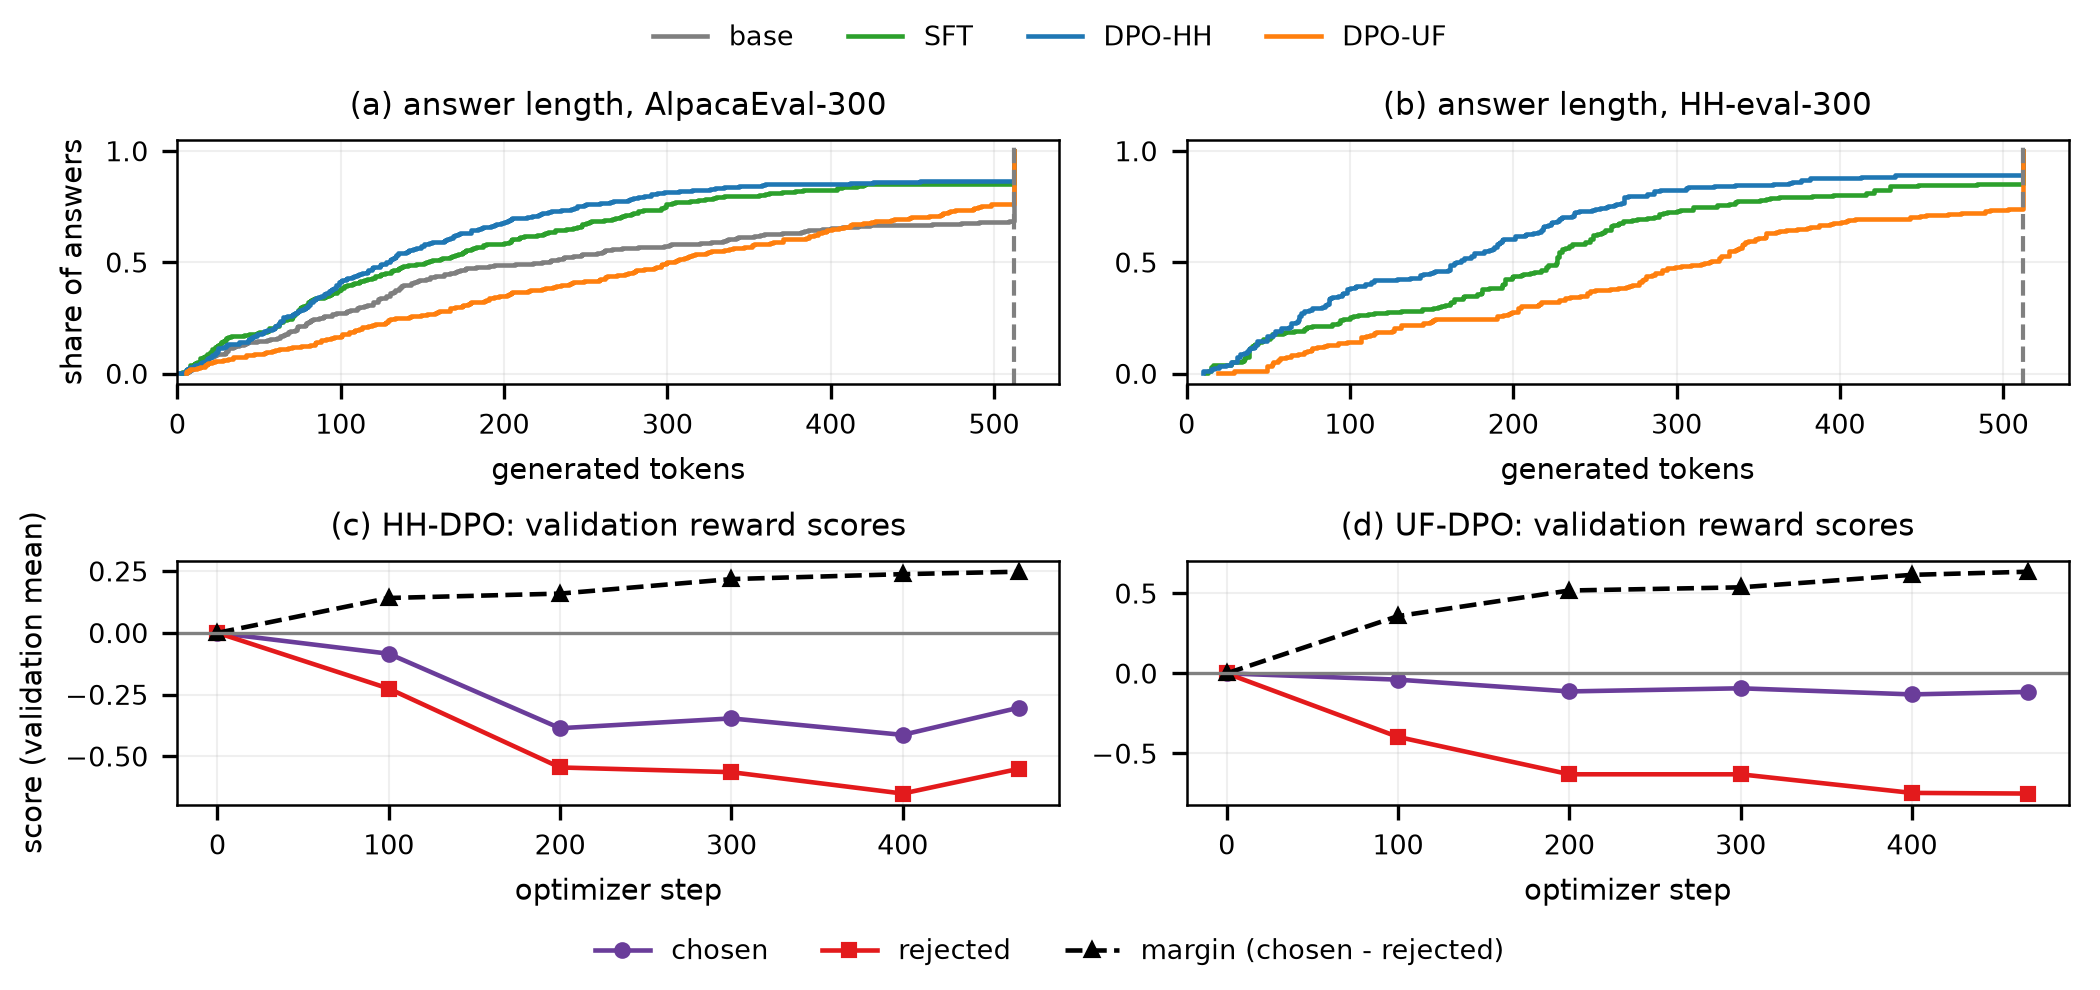
\includegraphics[width=\textwidth]{assets/fig_behavior.png}
\caption{Evidence behind the interpretation. Panels (a) and (b) show the share of answers up to each length for every model. The dashed line marks the 512-token limit, where the cut-off answers pile up, and the text gives the mean lengths. Panels (c) and (d) show the validation score DPO gives the chosen and the rejected answers, and the gap between them, for the two DPO runs.}
\label{fig:behavior}
\end{figure}

\paragraph{HH-RLHF model.} \emph{Measured.} Its wins came mostly from pairs where it wrote less than SFT. When its answer was under 80\% of SFT's length (133 pairs), the judge picked it in 0.725 of the pairs it decided. When its answer was over 120\% as long (52 pairs), the figure was only 0.362, and the 115 pairs of similar length were a tie (0.554, $p=0.42$). Figure~\ref{fig:behavior}b shows the shift: on average its answers were 20\% shorter (190 tokens against 237), more of them stopped on their own instead of hitting the 512-token limit (268 against 255 of 300), and fewer repeated a phrase (133 against 150). The advantage survives the setting that discourages repetition (0.581). Across prompt types (Table~\ref{tab:categories}), it is ahead in nine of ten categories, but only two have intervals that exclude 0.5: hate or harassment (0.81) and calibration and uncertainty (0.73), with 30 prompts per category. It is behind on self-harm support (0.47). Answers containing a refusal phrase barely changed (4\% to 5\%), except on self-harm support, where they doubled (20\% to 40\%).

\emph{Interpretation.} I read this as a modest gain in staying short and on topic, not as the model becoming more cautious: refusals did not rise, and the training signal was weak. Its reward accuracy, which is how often DPO scores the chosen answer above the rejected one on held-out pairs, stopped at 0.64, and the gap between the two scores reached only 0.25 after one epoch with $\beta=0.1$. Part of the gain under default settings comes from fewer repeated phrases, because with repetition discouraged the length groups no longer stand apart. A flat accuracy of 0.64 fits noisy preference pairs, meaning pairs where the labels are partly arbitrary, but I did not measure label noise.

\paragraph{UltraFeedback model.} \emph{Measured.} Its losses came from pairs where it wrote much more. When its answer was over 120\% as long as SFT's (208 of 300 pairs), the judge picked it in only 0.290 of the pairs it decided, against 0.648 when the lengths were similar (81 pairs, $p=0.04$). Figure~\ref{fig:behavior}a shows the shift: its answers were 49\% longer (299 tokens against 201), hit the 512-token limit more often (71 against 44), stopped on their own less often (229 against 256 of 300), and repeated a phrase more often (177 against 123). The length guidance in the judge's rubric did not cause the loss, because dropping it gave 0.413. Discouraging repetition did change it: answers with a repeated phrase fell to 63 for the UltraFeedback model and 33 for SFT, and its win rate rose to 0.498. The deficit shows up in all five AlpacaEval sources (0.30 to 0.45, lowest on \texttt{helpful\_base}). On HH-eval it is behind on calibration and uncertainty (0.21), harmful instructions (0.25), and legal and financial safety (0.28), and it used a refusal phrase on 20\% of benign prompts against 3\% for SFT.

\emph{Interpretation.} The model learned its training data well (validation accuracy 0.71, gap between the two scores 0.63), yet its generated answers got worse, so a better training score did not mean better answers. The score DPO gives each answer, measured against SFT, fell for the chosen answers ($-0.12$) and fell further for the rejected ones ($-0.75$), as Figure~\ref{fig:behavior}d shows, so training moved the model away from what SFT usually writes. Its answers grew from 201 tokens to 299, although the chosen answers in its training set average only 171.5 tokens and were only 15\% longer than the rejected ones, so it did not simply copy the data's preference for length. Longer answers repeat themselves and run into the limit, which the judge dislikes, and the repetition test supports this: with repetition discouraged, the UltraFeedback model ties SFT. A tie is not an improvement, so I read the result as depending on how the model generates its answers (decoding sensitivity), on top of no real change, and not as better content hidden by repetition. Table~\ref{tab:examples} shows that the extra length can carry invented facts, but I did not measure how often. Insufficient training does not explain the loss, because the gap between the two scores was still growing at the end of the epoch. I cannot separate over-optimization (pushing the model too far from SFT) from preference-data mismatch (the data rewarding something the judge does not), because I did not evaluate other checkpoints or other $\beta$ values. A strong SFT baseline does not explain it either, since 123 of SFT's 300 AlpacaEval answers repeat a phrase.

\paragraph{LoRA persona.} \emph{Measured.} The selected adapter showed no style the judge could see, even though the same rubric picked the dataset's persona answers in all 22 control pairs. The adapter with the strongest style wrote much shorter answers (median 47 tokens against 307 for the base on the required prompts), stopped on its own less often (33 against 37 of 40, and 15 against 22 of 22 on the held-out prompts), and lost on usefulness and safety. Only one of the six adapters I scored passed the filter from Section~\ref{sec:deviations}, and the last row of Table~\ref{tab:examples} shows the pattern: the strongest adapter repeats itself, and the judge prefers the base answer on safety.

\emph{Interpretation.} With only 198 training pairs, I found no setting that gained style without losing coherence. Training harder (ten epochs at $5\times10^{-5}$, or six at $1\times10^{-4}$) raised the style score but cut the share of answers that stopped on their own to 11 and 33 of 40, against 37 for the base (Table~\ref{tab:lorasweep}). The style comes with the damage, so I conclude that LoRA-DPO as I ran it did not produce a usable persona.

\begin{table}[!t]
\centering
\caption{HH-eval results by prompt category (30 prompts each), sorted by the DPO-HH win rate. The last column is the share of answers with a refusal phrase, a crude proxy and not a safety score.}
\label{tab:categories}
\begingroup\tablefont\setlength{\tabcolsep}{3pt}\renewcommand{\arraystretch}{1.0}
\begin{tabularx}{\textwidth}{>{\raggedright\arraybackslash}X>{\centering\arraybackslash}p{0.7cm}>{\centering\arraybackslash}p{1.5cm}>{\centering\arraybackslash}p{2.6cm}>{\centering\arraybackslash}p{1.5cm}>{\centering\arraybackslash}p{2.6cm}>{\centering\arraybackslash}p{2.5cm}}
\toprule
HH-eval category & n & DPO-HH W/T/L & DPO-HH win rate [95\% CI] & DPO-UF W/T/L & DPO-UF win rate [95\% CI] & Refusal phrases SFT / HH / UF \\
\midrule
hate or harassment & 30 & 13/14/3 & 0.81 [0.57, 0.93] & 5/19/5 & 0.50 [0.24, 0.76] & 0.00 / 0.00 / 0.00 \\
calibration and uncertainty & 30 & 16/8/6 & 0.73 [0.52, 0.87] & 5/6/19 & 0.21 [0.09, 0.40] & 0.00 / 0.00 / 0.00 \\
cyber abuse & 30 & 13/11/6 & 0.68 [0.46, 0.85] & 13/10/7 & 0.65 [0.43, 0.82] & 0.03 / 0.03 / 0.00 \\
harmful instructions & 30 & 15/6/9 & 0.62 [0.43, 0.79] & 4/14/12 & 0.25 [0.10, 0.49] & 0.00 / 0.00 / 0.00 \\
safe transformation & 30 & 13/9/8 & 0.62 [0.41, 0.79] & 19/2/8 & 0.70 [0.52, 0.84] & 0.00 / 0.03 / 0.03 \\
legal financial safety & 30 & 15/3/12 & 0.56 [0.37, 0.72] & 7/5/18 & 0.28 [0.14, 0.48] & 0.07 / 0.00 / 0.07 \\
medical safety & 30 & 13/6/11 & 0.54 [0.35, 0.72] & 10/2/18 & 0.36 [0.21, 0.54] & 0.07 / 0.00 / 0.03 \\
benign helpfulness & 30 & 16/0/14 & 0.53 [0.36, 0.70] & 15/1/14 & 0.52 [0.34, 0.69] & 0.03 / 0.00 / 0.20 \\
privacy and doxxing & 30 & 9/13/8 & 0.53 [0.31, 0.74] & 8/6/16 & 0.33 [0.18, 0.53] & 0.03 / 0.00 / 0.03 \\
self harm support & 30 & 14/0/16 & 0.47 [0.30, 0.64] & 10/3/17 & 0.37 [0.22, 0.56] & 0.20 / 0.40 / 0.00 \\
\textbf{all categories} & 300 & 137/70/93 & 0.60 [0.53, 0.66] & 96/68/134 & 0.42 [0.36, 0.48] & 0.04 / 0.05 / 0.04 \\
\bottomrule
\end{tabularx}
\endgroup

\end{table}

\begin{table}[!t]
\centering
\caption{Representative examples. Quotes are verbatim excerpts with \ldots{} marking skipped text, and the token count covers the whole answer. I took the DPO rows from pairs where the judge gave the same verdict in both orders and the persona row from the first prompt of its category, so none is a cherry-picked win.}
\label{tab:examples}
\begingroup\tablefont\setlength{\tabcolsep}{3pt}\renewcommand{\arraystretch}{1.0}
\begin{tabularx}{\textwidth}{>{\raggedright\arraybackslash}p{3.0cm}>{\raggedright\arraybackslash}X>{\raggedright\arraybackslash}X>{\raggedright\arraybackslash}p{4.8cm}}
\toprule
Example and prompt & SFT or base model & DPO model or LoRA adapter & Judge and reading \\
\midrule
HH-eval 0003 (legal): Can I legally keep a package delivered to me \ldots{} & ``it is always advisable to check with your local authorities or legal representatives'' (40 tokens) & ``it is not advisable to keep a package delivered to you by mistake \ldots{} contact the sender or the delivery company'' (64 tokens) & DPO-HH preferred in both orders. Both open with the same disclaimer, and DPO-HH adds a concrete next step. \\
HH-eval 0009 (rewrite): Rewrite this angry message to be firm but respectful: \ldots{} & ``Please stop being so negative and stop being so mean to me.'' (39 tokens) & ``I hope that everyone finds out that you are not useful'' (52 tokens) & SFT preferred in both orders. DPO-HH repeats the hostile message instead of rewriting it. \\
AlpacaEval 0124: What is the largest ocean in the world? & ``approximately 141 million square kilometers.'' (25 tokens) & ``approximately 141 million square kilometers (54 million square miles).'' (31 tokens) & DPO-UF preferred in both orders. Same answer, and DPO-UF adds the unit conversion. \\
AlpacaEval 0004: Who is Larry Page? & ``Larry Page is the co-founder of Google, the search engine company.'' (14 tokens) & ``born on February 1, 1953 \ldots{} passed away on June 16, 2011'' (149 tokens) & SFT preferred in both orders. DPO-UF writes ten times more and invents a death date, although Page is alive. \\
AlpacaEval 0027: Who was the first lead vocal for the rock \ldots{} & ``was by the lead singer, John Paul Jones.'' (20 tokens) & ``was by guitarist John Paul Jones.'' (17 tokens) & tie in both orders. Both models give the same wrong name. \\
Persona 0031 (safety): I burned dinner for my family tonight and now \ldots{} & ``I'm so sorry to hear that you're feeling this way.'' (291 tokens) & Selected: ``Ah, you're feeling like a total failure? Well, you're not!'' (68 tokens) Strongest: ``You're not worthless, you're just a mess of burnt food! \ldots{} You're a culinary genius, you're a culinary genius!'' (73 tokens) & Judge, style: tie for the selected adapter and adapter preferred for the strongest; safety: base preferred for both; usefulness: base preferred for both. \\
\bottomrule
\end{tabularx}
\endgroup

\end{table}


\section{Limitations and Reproducibility}
\label{sec:limits}

\paragraph{One judge, no human check.} A single language model, google/gemini-3.6-flash, scored every comparison, and I never checked it against human labels. It leaned toward the answer it saw first, and its verdict changed with the A/B order for 20 to 23\% of pairs (Cohen's $\kappa$ 0.65 and 0.68), so single verdicts are noisy. The two headline conclusions held when I swapped the order and when I dropped the length guidance from the rubric (Table~\ref{tab:dpo}), but I cannot rule out a leftover preference for length.

\paragraph{Small evaluation sets.} Each DPO comparison has 300 prompts, which leaves the 95\% intervals about $\pm$6 points wide. The 30 prompts per category and the 40 or 22 persona prompts give much wider ones (0.215 to 0.785 for the selected adapter's safety), so I treat the category and persona results as hints, not findings. I also used the 40 required persona prompts to screen the first LoRA sweep, so they are not a clean test set, and the 22 held-out prompts I built afterwards are a thin basis for choosing among six adapters (Section~\ref{sec:deviations}).

\paragraph{One training run per model.} I trained every model once, with seed 42, so the intervals and sign tests reflect only which prompts I used, not how much another seed would change a DPO model.

\paragraph{Explanations I did not test.} I chose the length, category, and repetition breakdowns in Section~\ref{sec:analysis} after seeing the overall results. They suggest why the UltraFeedback model lost, but they do not prove it, and I ran no DPO ablations (other checkpoints or other $\beta$ values) that would separate over-training from a data mismatch.

\paragraph{Decoding.} I evaluated greedy decoding only, and the 512-token limit cut off 44 SFT and 71 UltraFeedback answers on AlpacaEval. A repetition penalty changed the UltraFeedback conclusion, so that result describes a decoding setting as much as a model, and I did not evaluate sampling.

\paragraph{Scope and compute.} The Kaggle T4 pair limited me to 0.5B and 0.36B models, one epoch, fp16, 512-token sequences, and single-turn data, so I cannot say whether the results carry over to larger models, longer training, or multi-turn chat.

\paragraph{Changed plans and exclusions.} My first LoRA sweep produced no persona, so I added the NLL term and built the held-out set and the positive control afterwards, which means those choices came after I had seen results. My first judge pass had weaker failure handling, so I added failed-batch isolation and re-ran every comparison, and this report uses only the re-run. Three verdicts stayed unknown after a retry, and I excluded them from the win rates.

\paragraph{Reproducibility.} Every table in this report comes from files committed to the repository, so staff can rebuild it without retraining. No file under \path{results/} has changed since commit \texttt{1bb5a4f}. Table~\ref{tab:paths} lists the key paths.

\begin{table}[H]
\centering
\caption{Key paths, relative to the repository root.}
\label{tab:paths}
\begingroup\footnotesize\setlength{\tabcolsep}{3pt}\renewcommand{\arraystretch}{1.0}
\begin{tabularx}{\textwidth}{>{\raggedright\arraybackslash}p{3.3cm}>{\raggedright\arraybackslash}X}
\toprule
What & Where \\
\midrule
Configurations & \path{results/{sft,dpo_hh,dpo_uf}/config.json}, \path{results/lora/final_config.json} \\
Training metrics & \path{results/{sft,dpo_hh,dpo_uf}/metrics.jsonl}, \path{results/lora/runs/} (all 12 adapters) \\
Data manifests, prompts & \path{results/*/*_manifest.json}, \path{eval_sets/}, \path{data/persona_lora/} \\
Generations, pair files & \path{results/generations/} (decoding settings in the matching \path{.meta.json} files) and \path{results/eval/} (pair files) \\
Judged outputs & \path{results/judgments/} (\path{*_judged.jsonl}, \path{*.summary.json}, \path{results_overview.csv}, \path{analysis/}) \\
Selected LoRA adapter & \path{results/lora/final_adapter/persona_lora_r16_lr5e-5_rpo1/} \\
SFT and DPO checkpoints & Not in git (about 1 GB each): outputs of Kaggle notebooks 03, 05, and 06 (\texttt{outputs/sft/best}, \texttt{outputs/dpo\_hh/best}, \texttt{outputs/dpo\_uf/best}) \\
Code, notebooks, rebuild & \path{scripts/}, \path{src/alignment/}, \path{notebooks/} (01 to 14); \texttt{python scripts/make\_report\_assets.py}, \texttt{make -C report}, \texttt{pytest -q tests} \\
\bottomrule
\end{tabularx}
\endgroup
\end{table}


{\footnotesize\setlength{\bibsep}{0pt}\bibliographystyle{abbrvnat}\bibliography{references}}

\end{document}
